\documentclass[twocolumn,a4j]{jsarticle}
\setlength{\topmargin}{-20.4cm}
\setlength{\oddsidemargin}{-10.4mm}
\setlength{\evensidemargin}{-10.4mm}
\setlength{\textwidth}{18cm}
\setlength{\textheight}{26cm}

\usepackage[top=15truemm,bottom=20truemm,left=20truemm,right=20truemm]{geometry}
\usepackage[latin1]{inputenc}
\usepackage{amsmath}
\usepackage{amsfonts}
\usepackage{amssymb}
\usepackage[dvipdfmx]{graphicx}
\usepackage[hang,small,bf]{caption}
\usepackage[subrefformat=parens]{subcaption}
\usepackage[dvipdfmx]{color}
\usepackage{listings}
\usepackage{listings,jvlisting}
\usepackage{geometry}
\usepackage{framed}
\usepackage[dvipdfmx]{hyperref}
\usepackage{ascmac}
\usepackage{enumerate}
\usepackage{tabularx}
\usepackage{cancel}
\usepackage{scalefnt}
\usepackage{overcite}
\usepackage{otf}
\usepackage{multicol}
\usepackage[geometry]{ifsym}
\usepackage{array}

\renewcommand{\figurename}{Fig.}
\renewcommand{\tablename}{Table }

\lstset{
basicstyle={\ttfamily},
identifierstyle={\small},
commentstyle={\smallitshape},
keywordstyle={\small\bfseries},
ndkeywordstyle={\small},
stringstyle={\small\ttfamily},
frame={tb},
breaklines=true,
columns=[l]{fullflexible},
xrightmargin=0zw,
xleftmargin=3zw,
numberstyle={\scriptsize},
stepnumber=1,
numbersep=1zw,
lineskip=-0.5ex
}

% キャプション後ろのダブルコロンを消す
\makeatletter
\long\def\@makecaption#1#2{%
  \vskip\abovecaptionskip
  \iftdir\sbox\@tempboxa{#1\hskip1zw#2}%
    \else\sbox\@tempboxa{#1 #2}%
  \fi
  \ifdim \wd\@tempboxa >\hsize
    \iftdir #1\hskip1zw#2\relax\par
      \else #1 #2\relax\par\fi
  \else
    \global \@minipagefalse
    \hbox to\hsize{\hfil\box\@tempboxa\hfil}%
  \fi
  \vskip\belowcaptionskip}
\makeatother

% タイトル
\makeatletter
\def\@maketitle
{
\begin{center}
{\LARGE \@title \par}
\end{center}
\begin{flushright}
{\large \@date 報告書 No.38}\\
{\large M2 \@author}
\end{flushright}
\par\vskip 1.5em
}
\makeatother

\author{来代 勝胤}
\title{令和4年度 11月 第2週 報告書}
\date{2022/11/14}

\begin{document}
\columnseprule=0.1mm
\maketitle

\section*{報告内容}
\begin{enumerate}[1.]
  \item 数値シミュレーションの作成
  \item 車両モデルまわり流れの計測
  \item 来週の予定
\end{enumerate}

\section{数値シミュレーションの作成}

\subsection{粒子像の生成}
OpenFOAM を用いて,三角翼モデルの流れ場について数値解析を行い.
その流れ場から撮影シミュレーションを作成している.
シミュレーションで用いるバラメータは,
実際に撮影される較正ブロックの画像に近づくように設定する.

\begin{figure}[htbp]
  \centering
  \begin{tabular}{cc}
    \begin{minipage}[t]{0.45\hsize}
      \centering
      \includegraphics[keepaspectratio, width=40mm]{../images/Simulation/Calibration/simulation.bmp}
      \subcaption{Numerical simulation}
    \end{minipage} &
    \begin{minipage}[t]{0.45\hsize}
      \centering
      \includegraphics[keepaspectratio, width=40mm]{../images/Simulation/Calibration/experiment.bmp}
      \subcaption{Experiment}
    \end{minipage}
  \end{tabular}
  \caption{Image of calibration block}
\end{figure}

ピンホールカメラを想定し,現在は粒子画像の生成に取り組んでいる.
今後はこのデータにアルゴリズムを適用し,性能評価を行う.
\begin{figure}[htbp]
  \centering
  \begin{tabular}{cc}
    \begin{minipage}[t]{0.45\hsize}
      \centering
      \includegraphics[keepaspectratio, width=40mm]{../images/Simulation/Particles/simulation.bmp}
      \subcaption{Numerical simulation}
    \end{minipage} &
    \begin{minipage}[t]{0.45\hsize}
      \centering
      \includegraphics[keepaspectratio, width=40mm]{../images/Simulation/Particles/experiment.bmp}
      \subcaption{Experiment}
    \end{minipage}
  \end{tabular}
  \caption{Image of particles}
\end{figure}

\newpage
\subsection{数値シミュレーション結果と測定結果の比較}
今回の数値シミュレーションで使用した
三角翼モデルのシミュレーションについて
その解析結果と実際の測定結果の比較を行う.
また,数値シミュレーションはTable 1の条件で行い,
$x=0, 20, 40$ の位置の結果を示す.

\begin{table}[hbtp]
  \centering
  \caption{Condition of numerical simulation}
  \begin{tabular}{l c c}
    \hline
    Application      & OpenFOAM           \\ \hline
    Solver           & pimpleFoam         \\ \hline
    Turbulence model & $k-\omega$ SST     \\ \hline
    Time step        & 1/800          & s \\ \hline
    Simulation time  & 7.5            & s \\ \hline
  \end{tabular}
\end{table}

\begin{figure}[htbp]
  \centering
  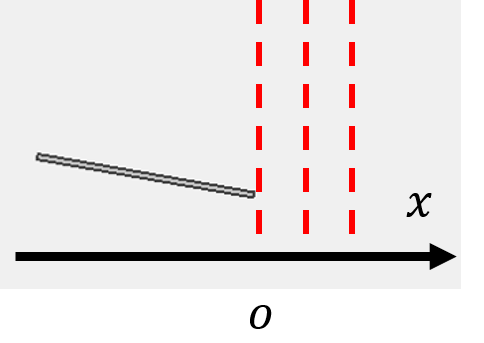
\includegraphics[keepaspectratio, width=45mm]{../images/measurement_plane_for_Delta_wingpng.png}
  \caption{Schematic of delta wing}
\end{figure}

\begin{figure}[htbp]
  \centering
  {
    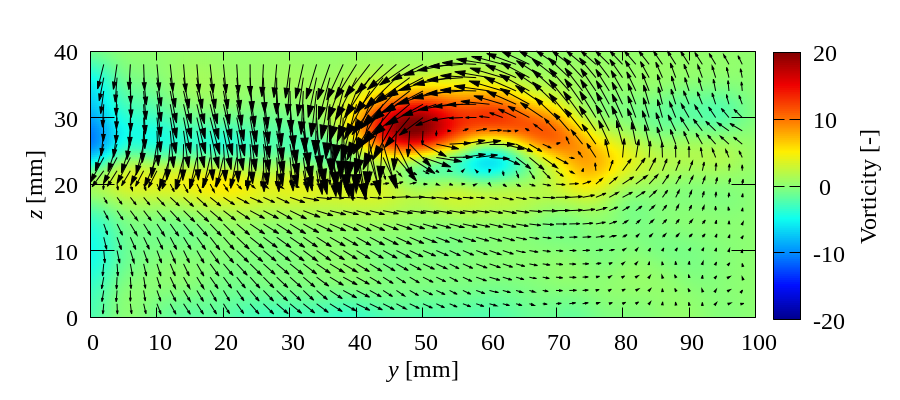
\includegraphics[keepaspectratio, width=80mm]{../images/Simulation/Compare/experiment_x=0.png}
    \subcaption{Experiment}
    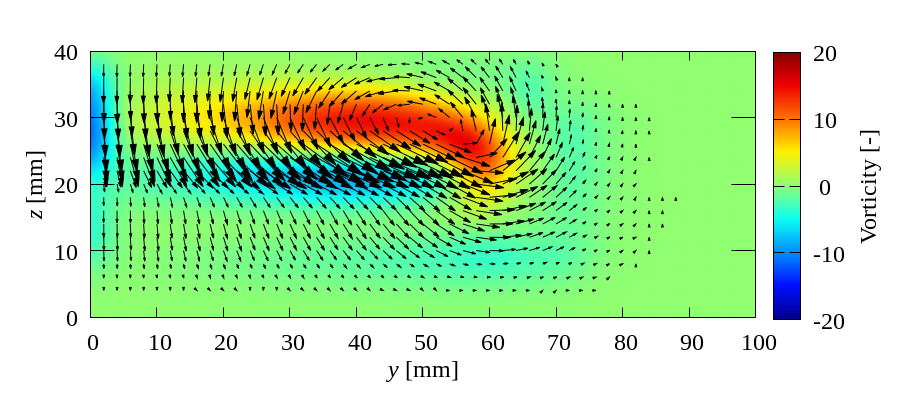
\includegraphics[keepaspectratio, width=80mm]{../images/Simulation/Compare/simulation_x=0.png}
    \subcaption{Simulation}
  }
  \caption{Delta wing :$x=0$}
\end{figure}

\newpage
\begin{figure}[htbp]
  \centering
  {
    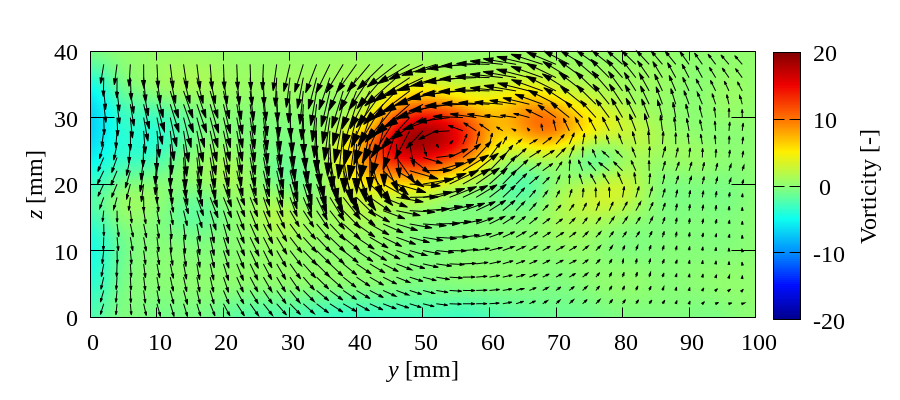
\includegraphics[keepaspectratio, width=80mm]{../images/Simulation/Compare/experiment_x=20.png}
    \subcaption{Experiment}
    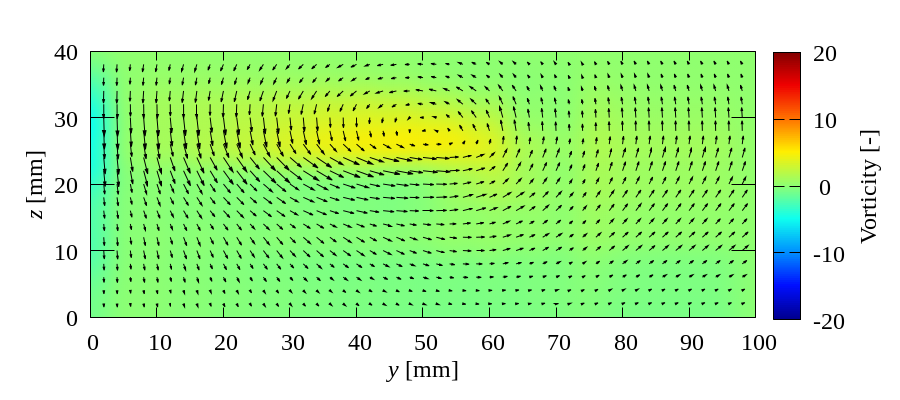
\includegraphics[keepaspectratio, width=80mm]{../images/Simulation/Compare/simulation_x=20.png}
    \subcaption{Simulation}
  }
  \caption{Delta wing :$x=20$}
  {
    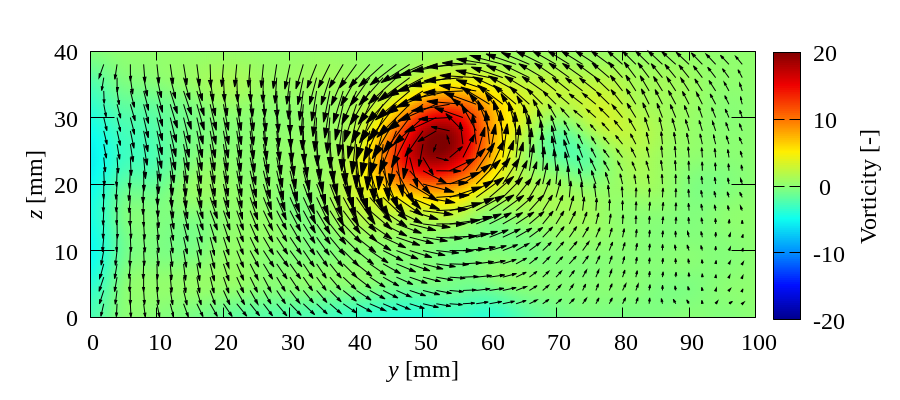
\includegraphics[keepaspectratio, width=80mm]{../images/Simulation/Compare/experiment_x=40.png}
    \subcaption{Experiment}
    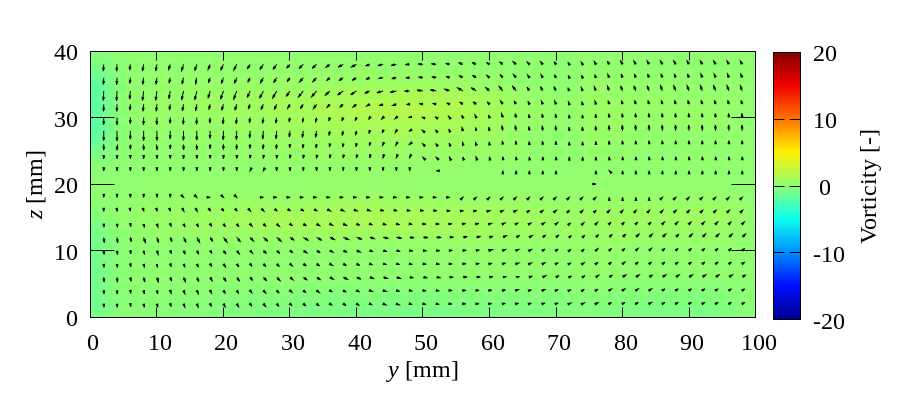
\includegraphics[keepaspectratio, width=80mm]{../images/Simulation/Compare/simulation_x=40.png}
    \subcaption{Simulation}
  }
  \caption{Delta wing :$x=40$}
\end{figure}

\newpage
\section{車両モデルまわり流れの計測}
車軸上を $x=0$ mm とし,$x=20$,$x=40$ の位置について計測を行った.
その解析結果を以下に示す.

\begin{figure}[htbp]
  \centering
  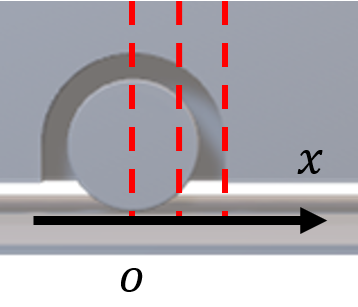
\includegraphics[keepaspectratio, width=35mm]{../images/measurement_plane_for_Vehicle_model.png}
  \caption{Schematic of vehicle model}
\end{figure}

\begin{figure}[htbp]
  \centering
  \begin{tabular}{cc}
    \begin{minipage}[t]{0.45\hsize}
      \centering
      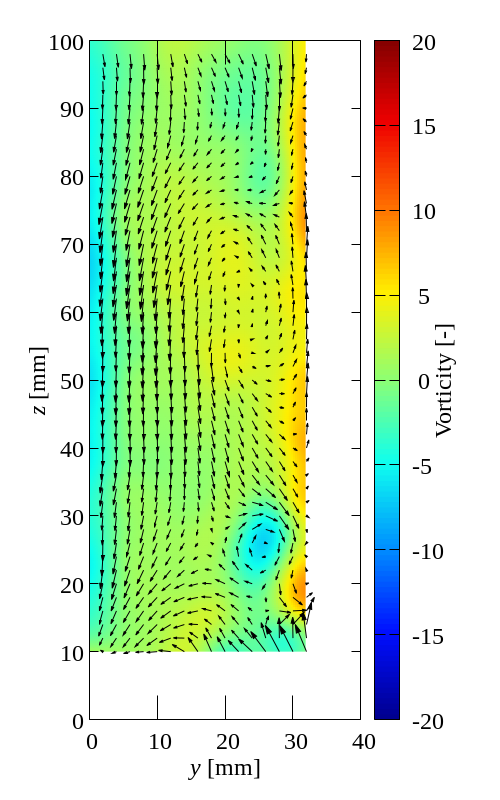
\includegraphics[keepaspectratio, width=44mm]{../images/stop_x=0.png}
      \subcaption{Without rotating}
    \end{minipage} &
    \begin{minipage}[t]{0.45\hsize}
      \centering
      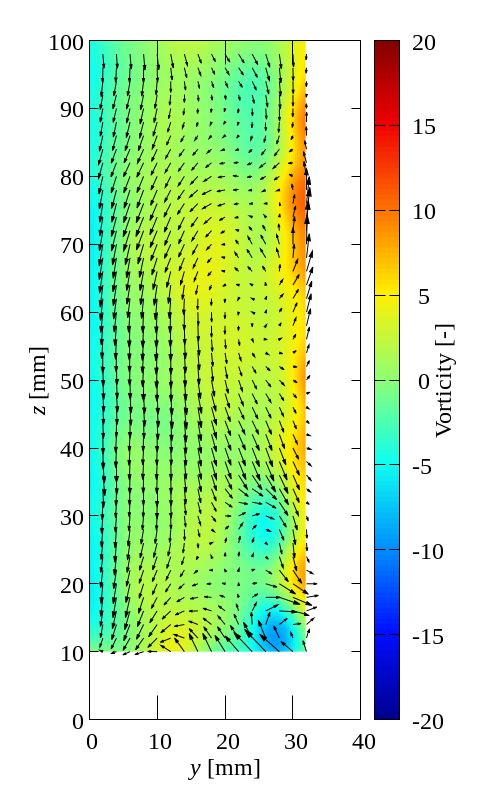
\includegraphics[keepaspectratio, width=44mm]{../images/rolling_x=0.png}
      \subcaption{With rotating}
    \end{minipage}
  \end{tabular}
  \caption{Vehicle model : $x=0$}
  \begin{tabular}{cc}
    \begin{minipage}[t]{0.45\hsize}
      \centering
      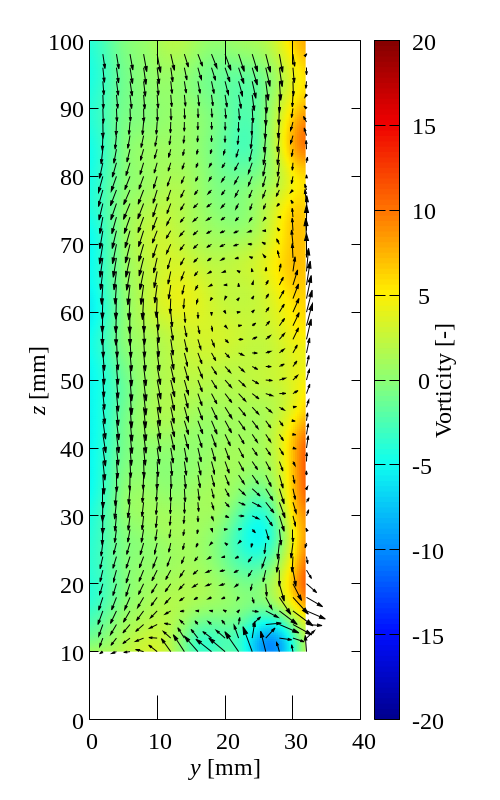
\includegraphics[keepaspectratio, width=44mm]{../images/stop_x=20.png}
      \subcaption{Without rotating}
    \end{minipage} &
    \begin{minipage}[t]{0.45\hsize}
      \centering
      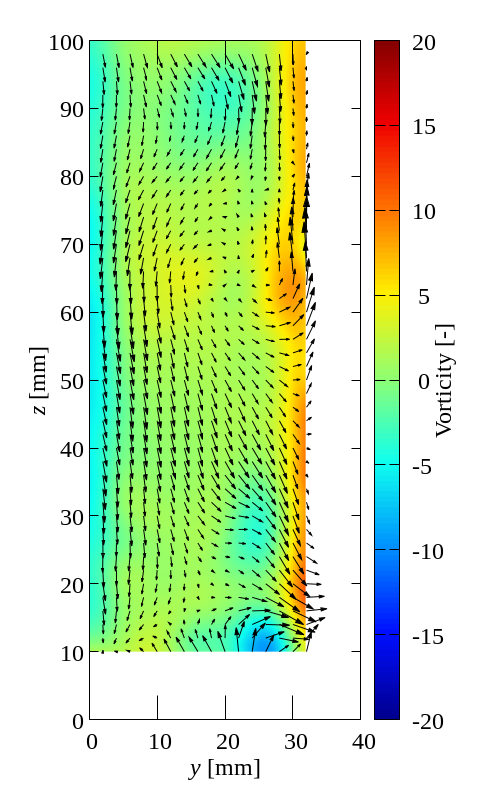
\includegraphics[keepaspectratio, width=44mm]{../images/rolling_x=20.png}
      \subcaption{With rotating}
    \end{minipage}
  \end{tabular}
  \caption{Vehicle model : $x=20$}
\end{figure}

\begin{figure}[htbp]
  \centering
  \begin{tabular}{cc}
    \begin{minipage}[t]{0.45\hsize}
      \centering
      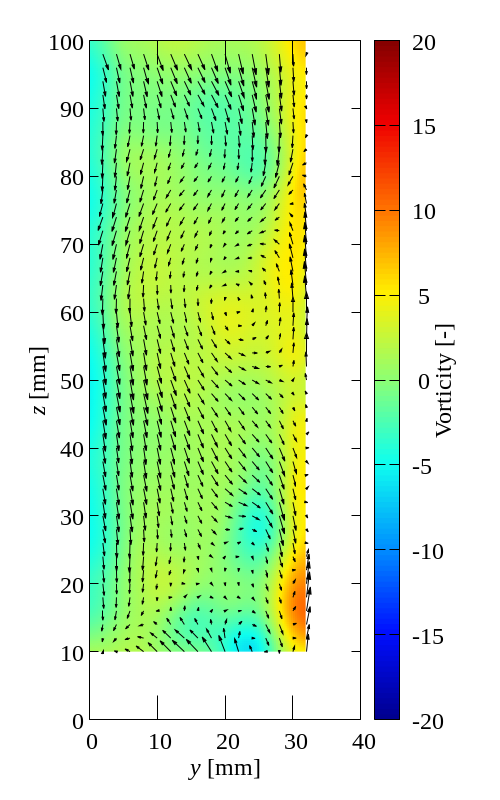
\includegraphics[keepaspectratio, width=44mm]{../images/stop_x=40.png}
      \subcaption{Without rotating}
    \end{minipage} &
    \begin{minipage}[t]{0.45\hsize}
      \centering
      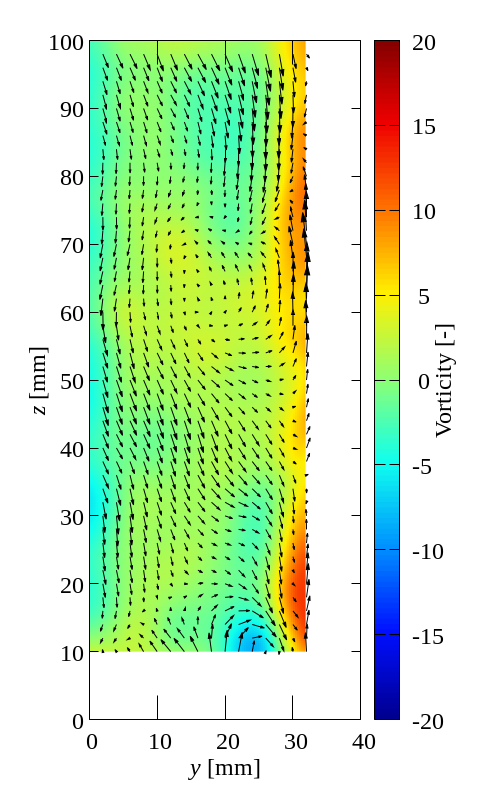
\includegraphics[keepaspectratio, width=44mm]{../images/rolling_x=40.png}
      \subcaption{With rotating}
    \end{minipage}
  \end{tabular}
  \caption{Vehicle model : $x=40$}
\end{figure}

\newpage
\subsection{粒子のペア数}
今回の解析結果において使用した
クラスタのペア数を調べる.
以下の数値は,1秒間当たりにレーザーシートを通過するペア数である.
これらの値より,描画に用いる格子点数 $50 \times 20$ 点に対して,
およそ20倍以上の粒子が存在することがわかる.
すなわち,格子点上の速度場を推測するにあたり,十分な速度ベクトルが存在するといえる.

\begin{table}[hbtp]
  \centering
  \caption{Number of cluster pair}
  \begin{tabular}{l c c}
    \hline
    with rolling    & $x=0$  & 22254.7 \\ \hline
    with rolling    & $x=20$ & 23130.8 \\ \hline
    with rolling    & $x=40$ & 21027.3 \\ \hline
    without rolling & $x=0$  & 24264.7 \\ \hline
    without rolling & $x=20$ & 24717.1 \\ \hline
    without rolling & $x=40$ & 23543.5 \\ \hline
  \end{tabular}
\end{table}

\newpage
\section{来週の予定}
\begin{itemize}
  \item 数値シミュレーションデータの解析
  \item 一様流データの利用方法検討
\end{itemize}

\end{document}